\documentclass[11pt,]{article}
\usepackage[T1]{fontenc}
\usepackage{lmodern}
\usepackage{amssymb,amsmath}
\usepackage{ifxetex,ifluatex}
\usepackage{fixltx2e} % provides \textsubscript
% use upquote if available, for straight quotes in verbatim environments
\IfFileExists{upquote.sty}{\usepackage{upquote}}{}
\ifnum 0\ifxetex 1\fi\ifluatex 1\fi=0 % if pdftex
  \usepackage[utf8]{inputenc}
\else % if luatex or xelatex
  \ifxetex
    \usepackage{mathspec}
    \usepackage{xltxtra,xunicode}
  \else
    \usepackage{fontspec}
  \fi
  \defaultfontfeatures{Mapping=tex-text,Scale=MatchLowercase}
  \newcommand{\euro}{€}
\fi
% use microtype if available
\IfFileExists{microtype.sty}{\usepackage{microtype}}{}
\usepackage[margin=1in]{geometry}
\usepackage{longtable,booktabs}
\usepackage{graphicx}
% Redefine \includegraphics so that, unless explicit options are
% given, the image width will not exceed the width of the page.
% Images get their normal width if they fit onto the page, but
% are scaled down if they would overflow the margins.
\makeatletter
\def\ScaleIfNeeded{%
  \ifdim\Gin@nat@width>\linewidth
    \linewidth
  \else
    \Gin@nat@width
  \fi
}
\makeatother
\let\Oldincludegraphics\includegraphics
{%
 \catcode`\@=11\relax%
 \gdef\includegraphics{\@ifnextchar[{\Oldincludegraphics}{\Oldincludegraphics[width=\ScaleIfNeeded]}}%
}%
\ifxetex
  \usepackage[setpagesize=false, % page size defined by xetex
              unicode=false, % unicode breaks when used with xetex
              xetex]{hyperref}
\else
  \usepackage[unicode=true]{hyperref}
\fi
\hypersetup{breaklinks=true,
            bookmarks=true,
            pdfauthor={},
            pdftitle={Modeling Lake Trophic State: A Data Mining Approach},
            colorlinks=true,
            citecolor=blue,
            urlcolor=blue,
            linkcolor=magenta,
            pdfborder={0 0 0}}
\urlstyle{same}  % don't use monospace font for urls
\setlength{\parindent}{0pt}
\setlength{\parskip}{6pt plus 2pt minus 1pt}
\setlength{\emergencystretch}{3em}  % prevent overfull lines
\setcounter{secnumdepth}{5}

\title{Modeling Lake Trophic State: A Data Mining Approach}
\author{}
\date{}

\begin{document}

\begin{center}
\huge Modeling Lake Trophic State: A Data Mining Approach \\[0.2cm]
\normalsize
\end{center}


\emph{US Environmental Protection Agency, Office of Research and
Development, National Health and Environmental Effects Research
Laboratory, Atlantic Ecology Division, 27 Tarzwell Drive Narragansett,
RI, 02879, USA}

\emph{corresponding
author:\href{mailto:hollister.jeff@epa.gov}{hollister.jeff@epa.gov}}

\begin{singlespace}
\begin{abstract}
Productivity of lentic ecosystems has been well studied and it is widely accepted that as nutrient inputs increase,  productivity increases and lakes transition from low trophic state (e.g. oligotrophic) to higher trophic states  (e.g. eutrophic). These broad trophic state classifications are good predictors of ecosystem health and ecosystem services/disservices (e.g. recreation, aesthetics, fisheries, and harmful algal blooms). While the relationship between  nutrients and trophic state provides reliable predictions, it requires *in situ* water quality data in order to paramterize the model.  This limits the application of these models to lakes with existing and, more importanly, available water quality data.  To expand our ability to predict in lakes without water quality data, we take advantage of the availability of a large national lakes water quality database, land use/land cover data, lake morphometry data, other universally available data, and modern data mining approaches to build and assess models of lake tropic state that may be more universally applied.  We use random forests and random forest variable selection to identify variables to be used for predicting trophic state and we compare the performance of two models of trophic state (as determined by chlorophyll *a* concentration).   The first model estimates trophic state with *in situ* as well as universally available data and the second model uses universally available data only. For each of these models we used three separate trophic state categories, for a total of six models. Overall accuracy for the *in situ* and universal data models ranged from xx% to xx% and xx, xx, and xx described the most variation in trophic state.  For the universal data only models, Overall accuraccy ranged from xx% to xx% and xx, xx, and xx described the most variation in trophic state. Lastly, it is believed that the presence and abundance of cyanobacteria is strongly associated with trophic state.  To test this we examine the association between estimates of cyanobacteria biovolume and the measured and predicted trophic state.  Expanding these preliminary results to include cyanobacteria taxa indicates that cyanobacteria are significantly more likely to be found in highly eutrophic lakes. These results suggest that predictive models of lake trophic state may be improved with additional information on the landscape surrounding lakes and that those models provide additional information on the presence of potentially harmful cyanobacteria taxa. 
\end{abstract}
\end{singlespace}

\section{Introduction}\label{introduction}

Productivity in lentic systems is often categorized across a range of
tropic states (e.g.~the tropic continuum) from early succesional
(i.e.~oligotrophic)to late successional lakes (i.e.~hypereutrophic)
(Carlson 1977). Lakes naturally occur across the range of trophic state
and higher primary productivity is not necessarily a predictor of poor
ecological condition. Lakes that are naturally oligotrophic occur in
nutrient poor areas or have a more recent geologic history. These lakes
are often found in higher elevations, have clear water, and are often
favored for drinking water or direct contact recreation (e.g.~swimming).
Lakes with higher productivity (e.g.~eutrophic lakes) have greater
nutrient loads, tend to be less clear, have greater density of aquatic
plants, and often support more diverse and abundant fish communities.
Lakes will naturally shift to higher trophic states but this is a slow
process. Given this fact, monitoring trophic state allows the
identification of rapid shifts in trophic state or locating lakes with
unusually high productivity (e.g.~hypereutrophic). These cases are
indicative of lakes under greater anthropogenic nutrient loads, also
known as cultural eutrophication, and are more likely to be at risk of
fish kills, fouling, and harmful algal blooms(Smith 1998, Smith et al.
1999, 2006). Given the association between trophic state and many
ecosystem services and disservices, being able to model trophic state
could allow for estimating trophic state in unmonitored lakes and
provide a first cut at identifying lakes with the potential for harmful
algal blooms and other problems associated with cultural eutrophication.

Cyanobacteria are an important taxonomic group associated with harmful
algal blooms in lakes. Understanding the drivers of cyanobacteria
presence has important implications for lake management and for the
protection of human and ecosystem health. Chlorophyll a concentration, a
measure of the biological productivity of a lake, is one such driver and
is largely, although not exclusively, determined by nutrient inputs. As
nutrient inputs increase, productivity increases and lakes transition
from low trophic state (e.g.~oligotrophic) to higher trophic states
(e.g.~hypereutrophic). These broad trophic state classifications are
associated with ecosystem health and ecosystem services/disservices
(e.g.~recreation, aesthetics, fisheries, and harmful algal blooms).
Thus, models of trophic state might be used to predict things like
cyanobacteria.

We have three goals for this preliminary research. First, we build and
assess multiple models of lake trophic state using a full suite of data
including \emph{in situ} water quality and universally available data
(e.g.~landscape data). Second, we assess the accuracy of predicted
trophic state in lakes with only the universally available data. Lastly,
we explore associations between trophic state and cyanobacteria to
explore.

\section{Methods}\label{methods}

\subsection{Data and Study Area}\label{data-and-study-area}

We utilize four primary sources of data for this study,the National
Lakes Assessment (NLA), the National Lake Cover Dataset (NLCD), modeled
lake morphometery, and estimated cyanobacteria biovolumes (Homer et al.
2004, USEPA 2009, Xian et al. 2009, Hollister and Milstead 2010,
Hollister et al. 2011, Beaulieu et al. 2013, Hollister 2014). All
datasets are national in scale and provide a unique snapshot view of the
condition of lakes in the United States'.

The NLA data were collected during the summer of 2007 and the final data
were released in 2009. With consistent methods and metrics collected at
1056 locations across the conterminous United States (Figure
\ref{fig:nlaMap}), the NLA provides a unique opportunity to examine
broad scale patterns in lake productivity. The NLA collected data on
biophysical measures of lake water quality and habitat. For this
analysis we primarily examined the water quality measurements from the
NLA (USEPA 2009). Adding to the monitoring data collected via the NLA,
we use the 2006 NLCD data to examine the possible landscape-level
drivers of trophic status in lakes. The NLCD is a nationally collected
land use land cover dataset that also provides estimates of impervious
surface. We collected total land use land cover and total percent
impervious surface within a 3 kilometer buffer surrounding the lake to
examine larger landscape-level effect (Homer et al. 2004, Xian et al.
2009). We also used various measures of lake morphometry (i.e.~depth,
volume, fetch, etc.) as they are important in understanding lake
productivity, yet many of these data are difficult to obtain for large
numbers of lakes over broad regions. To add this information we modeled
lake morphometry (Hollister and Milstead 2010, {\textbf{???}}, Hollister
et al. 2011, Hollister 2014). Lastly, to explore associations between
trophic state and cyanobacteria, we used estimates of cyanobacterial
biovoulme caluclated by Beaulieu \emph{et al.} (2013). Cyanobacteria
biovolumes are a truer measure of cyanobacteria dominance than abundance
as there is great variability in the size within and between species. We
have consolidated the taxa level estimates from Beaulieu \emph{et al.}
(2013) and summed that information on a per-lake basis.

\begin{figure}[htbp]
\centering
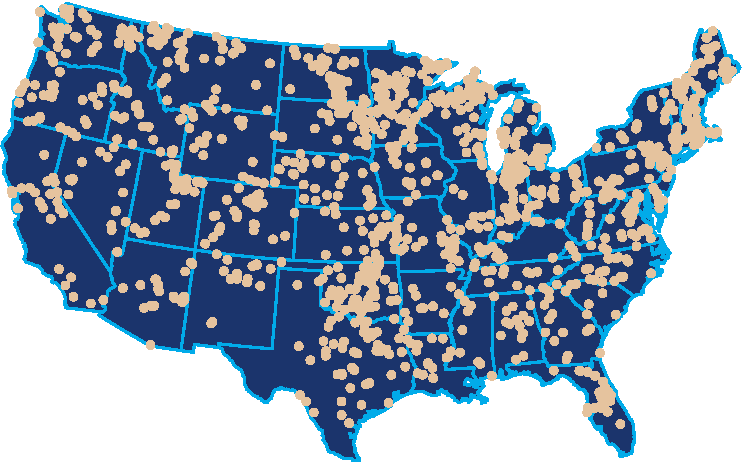
\includegraphics{./manuscript_files/figure-latex/nlaMap.pdf}
\caption{Map of the distribution of National Lakes Assesment Sampling
locations\label{fig:nlaMap}}
\end{figure}

\subsection{Predicting Trophic State with Random
Forests}\label{predicting-trophic-state-with-random-forests}

Random forest is a machine learning algorithm that aggregates numerous
decision trees in order to obtain a consensus prediction of the response
categories (Breiman 2001). Bootstrapped sample data is recursively
partitioned according to a given random subset of predictor variables
and completely grown without pruning. With each new tree, both the
sample data and predictor variable subset is randomly selected.

While random forests are able to handle numerous correlated variables
without a decrease in prediction accuracy, unusually large numbers of
related variables can reduce accuracy and increase the chances of
over-fitting the model. This is a problem often faced in gene selection
and in that field, a variable selection method based on random forest
has been succesfully applied (D{í}az-Uriarte and De Andres 2006). We use
varselRF in R to initially examine the importance of the water quality
and GIS derived variables and select a subset, the reduced model, to
then pass to random forest(Diaz-Uriarte 2010).

Using R's randomForest package, we pass the reduced models selected with
varSelRF and calculate confusion matrices, overall accuracy and kappa
coeffecient (Liaw and Wiener 2002). From the reduced model random
forests we collect a consensus prediction and calculate a confusion
matrix and summary stats.

\subsection{Model Details}\label{model-details}

Using a combination of the \texttt{varSelRF} and \texttt{randomForest}
we ran models for six combinations of variables and trophic state
classifications. These combinations included different combinations of
the Chlorphyll \emph{a} trophic states (Table
\ref{tab:trophicStateTable}) along with all variables and the GIS only
variables (i.e.~no \emph{in situ} infromation). The six model
combinations were:

\begin{enumerate}
\def\labelenumi{\arabic{enumi}.}
\itemsep1pt\parskip0pt\parsep0pt
\item
  Chlorophyll \emph{a} trophic state - 4 class = All variables (\emph{in
  situ} water quality, lake morphometry, and landscape)
\item
  Chlorophyll \emph{a} trophic state - 3 class = All variables (\emph{in
  situ} water quality, lake morphometry, and landscape)
\item
  Chlorophyll \emph{a} trophic state - 2 class = All variables (\emph{in
  situ} water quality, lake morphometry, and landscape)
\item
  Chlorophyll \emph{a} trophic state - 4 class = All variables (lake
  morphometry, and landscape)
\item
  Chlorophyll \emph{a} trophic state - 3 class = All variables (lake
  morphometry, and landscape)
\item
  Chlorophyll \emph{a} trophic state - 2 class = All variables (lake
  morphometry, and landscape)
\end{enumerate}

\begin{longtable}[c]{@{}llll@{}}
\toprule\addlinespace
Trophic State (4) & Trophic State (3) & Trophic State (2) & Cut-off
\\\addlinespace
\midrule\endhead
oligo & oligo & oligo/meso & \textless{}= 0.2
\\\addlinespace
meso & meso/eu & oligo/meso & \textgreater{}2-7
\\\addlinespace
eu & meso/eu & eu/hyper & \textgreater{}7-30
\\\addlinespace
hyper & hyper & eu/hyper & \textgreater{}30
\\\addlinespace
\bottomrule
\addlinespace
\caption{Chlorophyll a based trophic state
cut-offs\label{tab:trophicStateTable}}
\end{longtable}

\section{Results}\label{results}

\subsection{Model 1: 4 Trophic States \textasciitilde{} All
Variables}\label{model-1-4-trophic-states-all-variables}

The selected variables that made up Model 1 were Potassium,
Nitrogen:Phosphorus, Total Nitrogen, Total Phosphorus, Total Organic
Carbon, Turbidity, Ecoregion, Organic Ions, Dissolved Organic Carbon,
and Maximum Lake Depth (Table \ref{tab:VarSel_Model1}). Total accuracy
for Model 1 is 0.667\% and the Cohen's Kappa is 0.546 (Table
\ref{tab:Confusion_Model1}).

\begin{longtable}[c]{@{}lr@{}}
\toprule\addlinespace
Variable & Percent
\\\addlinespace
\midrule\endhead
K & 1.00
\\\addlinespace
NPratio & 1.00
\\\addlinespace
NTL & 1.00
\\\addlinespace
PTL & 1.00
\\\addlinespace
TOC & 1.00
\\\addlinespace
TURB & 1.00
\\\addlinespace
WSA\_ECO9 & 1.00
\\\addlinespace
ORGION & 0.29
\\\addlinespace
DOC & 0.18
\\\addlinespace
DEPTHMAX & 0.03
\\\addlinespace
\bottomrule
\addlinespace
\caption{Variable selection results for Model
1\label{tab:VarSel_Model1}}
\end{longtable}

\begin{longtable}[c]{@{}lllll@{}}
\toprule\addlinespace
Oligo & Meso & Eu & Hyper & class.error
\\\addlinespace
\midrule\endhead
135 & 58 & 4 & 1 & 0.32
\\\addlinespace
42 & 235 & 76 & 9 & 0.35
\\\addlinespace
2 & 70 & 217 & 47 & 0.35
\\\addlinespace
0 & 3 & 68 & 175 & 0.29
\\\addlinespace
\bottomrule
\addlinespace
\caption{Random Forest confusion matrix for Model
1\label{tab:Confusion_Model1}}
\end{longtable}

Lastly, tubidity, total phosphorus, total nitrogen, and total organic
carbon were the most important predictors of the 4 classes of trophic
state (Figure \ref{fig:Importance_Model1}).

\begin{figure}[htbp]
\centering
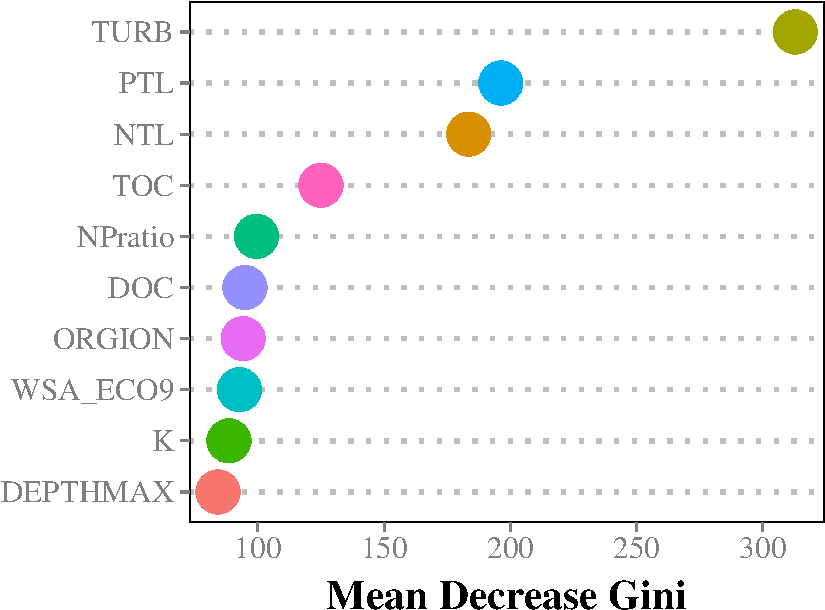
\includegraphics{./manuscript_files/figure-latex/Importance_Model1.pdf}
\caption{Importance plot for Model 1\label{fig:Importance_Model1}}
\end{figure}

\subsection{Model 2: 3 Trophic States \textasciitilde{} All
Variables}\label{model-2-3-trophic-states-all-variables}

Total accuracy for Model 2 is 0.799\% and the Cohen's Kappa is 0.618.

\begin{longtable}[c]{@{}lr@{}}
\toprule\addlinespace
Variable & Percent
\\\addlinespace
\midrule\endhead
DOC & 1.00
\\\addlinespace
K & 1.00
\\\addlinespace
NTL & 1.00
\\\addlinespace
ORGION & 1.00
\\\addlinespace
PTL & 1.00
\\\addlinespace
TOC & 1.00
\\\addlinespace
TURB & 1.00
\\\addlinespace
WSA\_ECO9 & 1.00
\\\addlinespace
DEPTHMAX & 0.98
\\\addlinespace
NPratio & 0.76
\\\addlinespace
AlbersX & 0.48
\\\addlinespace
CropsPer\_3000m & 0.27
\\\addlinespace
ELEV\_PT & 0.16
\\\addlinespace
AlbersY & 0.05
\\\addlinespace
NH4 & 0.05
\\\addlinespace
PH\_FIELD & 0.01
\\\addlinespace
EvergreenPer\_3000m & 0.01
\\\addlinespace
\bottomrule
\addlinespace
\caption{Variable selection results for Model 2}
\end{longtable}

\begin{longtable}[c]{@{}llll@{}}
\toprule\addlinespace
Oligo & Meso/Eu & Hyper & class.error
\\\addlinespace
\midrule\endhead
121 & 75 & 0 & 0.38
\\\addlinespace
40 & 609 & 40 & 0.12
\\\addlinespace
0 & 72 & 173 & 0.29
\\\addlinespace
\bottomrule
\addlinespace
\caption{Random Forest confusion matrix for Model 2}
\end{longtable}

\begin{figure}[htbp]
\centering
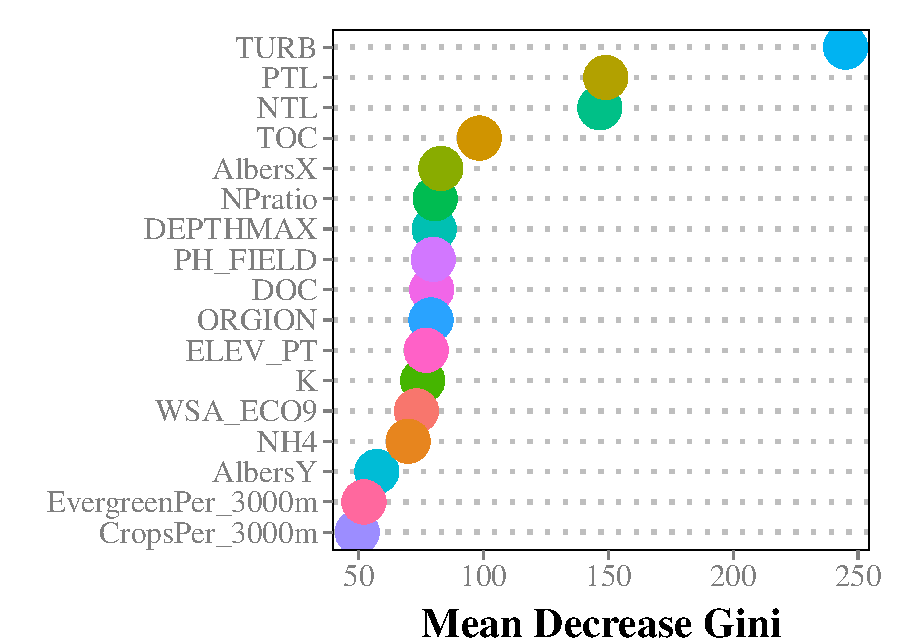
\includegraphics{./manuscript_files/figure-latex/Importance_Model2.pdf}
\caption{Importance plot for Model 2}
\end{figure}

\subsection{Model 3: 2 Trophic States \textasciitilde{} All
Variables}\label{model-3-2-trophic-states-all-variables}

Total accuracy for Model 3 is 0.87\% and the Cohen's Kappa is 0.741.

\begin{longtable}[c]{@{}lr@{}}
\toprule\addlinespace
Variable & Percent
\\\addlinespace
\midrule\endhead
K & 1.00
\\\addlinespace
NPratio & 1.00
\\\addlinespace
NTL & 1.00
\\\addlinespace
PTL & 1.00
\\\addlinespace
TOC & 1.00
\\\addlinespace
TURB & 1.00
\\\addlinespace
WSA\_ECO9 & 1.00
\\\addlinespace
ORGION & 0.99
\\\addlinespace
DEPTHMAX & 0.96
\\\addlinespace
DDs45 & 0.90
\\\addlinespace
ELEV\_PT & 0.85
\\\addlinespace
DOC & 0.58
\\\addlinespace
AlbersX & 0.06
\\\addlinespace
AlbersY & 0.03
\\\addlinespace
Na & 0.03
\\\addlinespace
\bottomrule
\addlinespace
\caption{Variable selection results for Model 3}
\end{longtable}

\begin{longtable}[c]{@{}lll@{}}
\toprule\addlinespace
Oligo/Meso & Eu/Hyper & class.error
\\\addlinespace
\midrule\endhead
489 & 71 & 0.13
\\\addlinespace
77 & 505 & 0.13
\\\addlinespace
\bottomrule
\addlinespace
\caption{Random Forest confusion matrix for Model 3}
\end{longtable}

\begin{figure}[htbp]
\centering
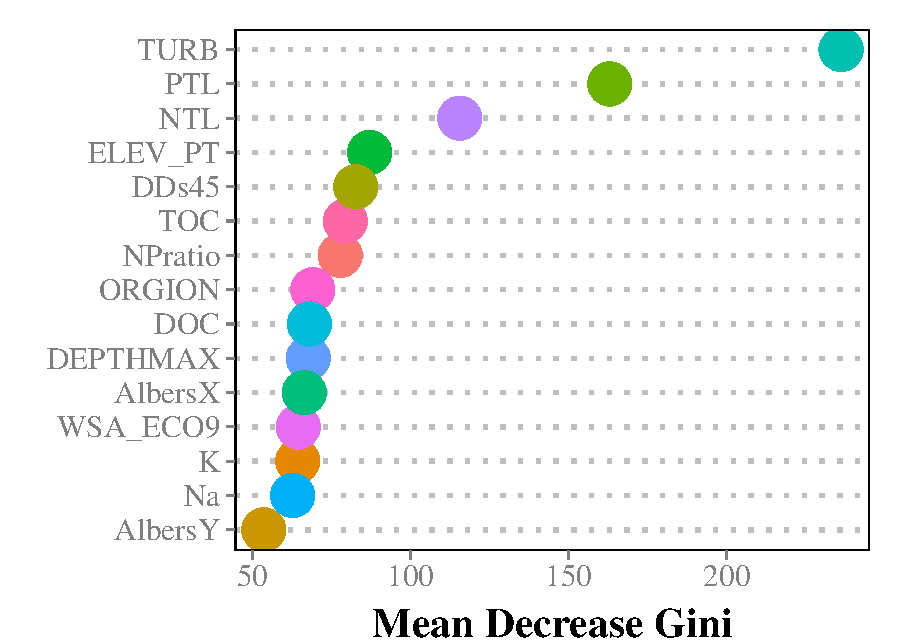
\includegraphics{./manuscript_files/figure-latex/Importance_Model3.pdf}
\caption{Importance plot for Model 3}
\end{figure}

\subsection{Model 4: 4 Trophic States \textasciitilde{} GIS Only
Variables}\label{model-4-4-trophic-states-gis-only-variables}

Total accuracy for Model 4 is 0.482\% and the Cohen's Kappa is 0.292.

\begin{longtable}[c]{@{}lr@{}}
\toprule\addlinespace
Variable & Percent
\\\addlinespace
\midrule\endhead
AlbersX & 1.00
\\\addlinespace
CropsPer\_3000m & 1.00
\\\addlinespace
EvergreenPer\_3000m & 1.00
\\\addlinespace
MeanDepthCorrect & 1.00
\\\addlinespace
WSA\_ECO9 & 1.00
\\\addlinespace
AlbersY & 0.35
\\\addlinespace
ELEV\_PT & 0.02
\\\addlinespace
\bottomrule
\addlinespace
\caption{Variable selection results for Model 4}
\end{longtable}

\begin{longtable}[c]{@{}lllll@{}}
\toprule\addlinespace
Oligo & Meso & Eu & Hyper & class.error
\\\addlinespace
\midrule\endhead
95 & 73 & 27 & 2 & 0.52
\\\addlinespace
48 & 201 & 80 & 32 & 0.44
\\\addlinespace
20 & 114 & 124 & 77 & 0.63
\\\addlinespace
2 & 36 & 79 & 129 & 0.48
\\\addlinespace
\bottomrule
\addlinespace
\caption{Random Forest confusion matrix for Model 4}
\end{longtable}

\begin{figure}[htbp]
\centering
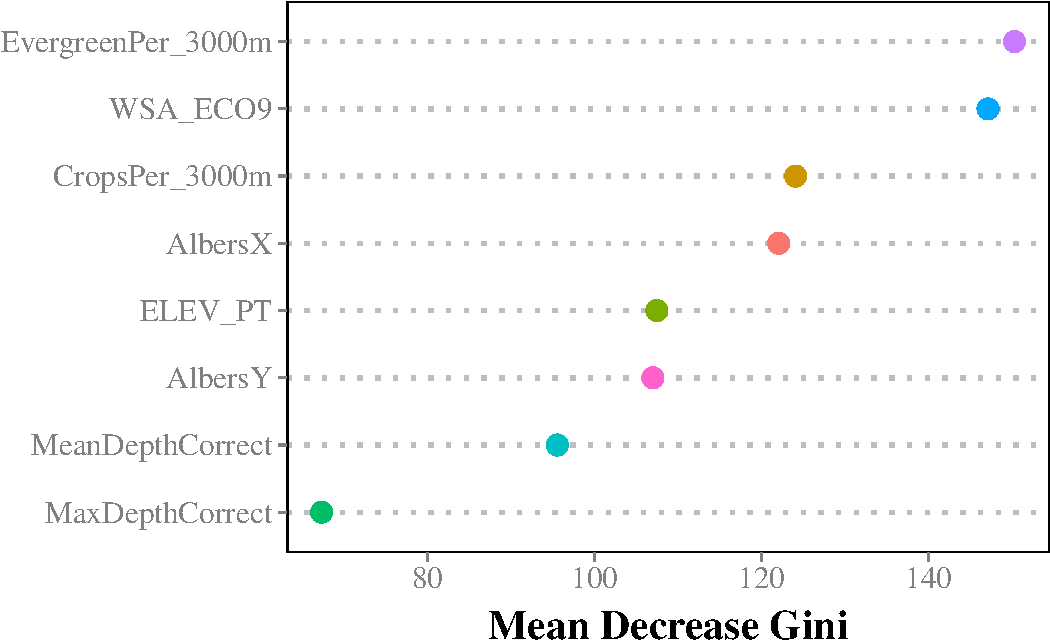
\includegraphics{./manuscript_files/figure-latex/Importance_Model4.pdf}
\caption{plot of chunk Importance\_Model4}
\end{figure}

:Importance plot for Model 4

\subsection{Model 5: 3 Trophic States \textasciitilde{} GIS Only
Variables}\label{model-5-3-trophic-states-gis-only-variables}

Total accuracy for Model 5 is 0.673\% and the Cohen's Kappa is 0.343.

\begin{longtable}[c]{@{}lr@{}}
\toprule\addlinespace
Variable & Percent
\\\addlinespace
\midrule\endhead
AlbersX & 1.00
\\\addlinespace
AlbersY & 1.00
\\\addlinespace
CropsPer\_3000m & 1.00
\\\addlinespace
EvergreenPer\_3000m & 1.00
\\\addlinespace
MaxDepthCorrect & 1.00
\\\addlinespace
MeanDepthCorrect & 1.00
\\\addlinespace
WSA\_ECO9 & 1.00
\\\addlinespace
ELEV\_PT & 0.97
\\\addlinespace
DeciduousPer\_3000m & 0.94
\\\addlinespace
ShrubPer\_3000m & 0.21
\\\addlinespace
WoodyWetPer\_3000m & 0.11
\\\addlinespace
DevOpenPer\_3000m & 0.10
\\\addlinespace
VolumeCorrect & 0.04
\\\addlinespace
\bottomrule
\addlinespace
\caption{Variable selection results for Model 5}
\end{longtable}

\begin{longtable}[c]{@{}llll@{}}
\toprule\addlinespace
Oligo & Meso/Eu & Hyper & class.error
\\\addlinespace
\midrule\endhead
79 & 116 & 1 & 0.6
\\\addlinespace
48 & 582 & 66 & 0.16
\\\addlinespace
0 & 141 & 105 & 0.57
\\\addlinespace
\bottomrule
\addlinespace
\caption{Random Forest confusion matrix for Model 5}
\end{longtable}

\begin{figure}[htbp]
\centering
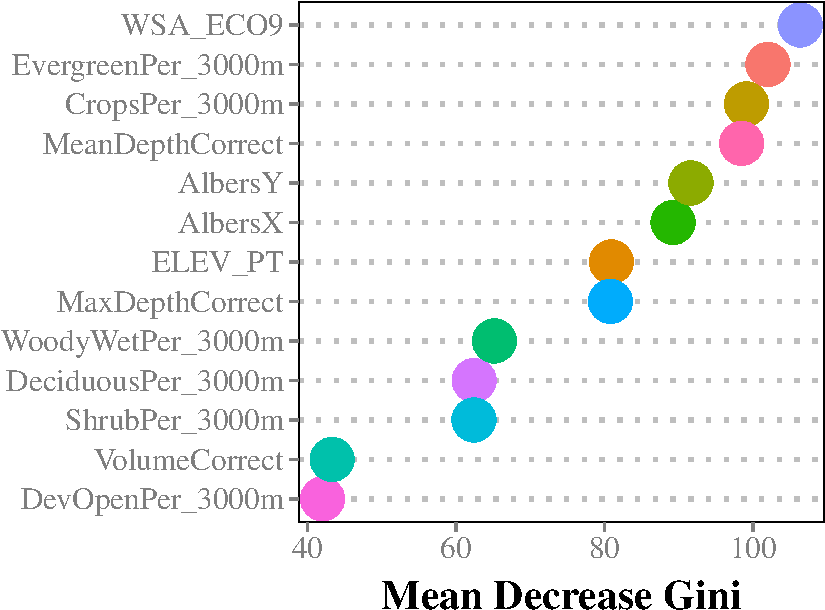
\includegraphics{./manuscript_files/figure-latex/Importance_Model5.pdf}
\caption{Importance plot for Model 5}
\end{figure}

\subsection{Model 6: 2 Trophic States \textasciitilde{} GIS Only
Variables}\label{model-6-2-trophic-states-gis-only-variables}

Total accuracy for Model 6 0.758\% and the Cohen's Kappa is 0.517.

\begin{longtable}[c]{@{}lr@{}}
\toprule\addlinespace
Variable & Percent
\\\addlinespace
\midrule\endhead
AlbersX & 1.00
\\\addlinespace
CropsPer\_3000m & 1.00
\\\addlinespace
DDs45 & 1.00
\\\addlinespace
ELEV\_PT & 1.00
\\\addlinespace
EvergreenPer\_3000m & 1.00
\\\addlinespace
MeanDepthCorrect & 1.00
\\\addlinespace
WSA\_ECO9 & 1.00
\\\addlinespace
AlbersY & 0.98
\\\addlinespace
MaxDepthCorrect & 0.98
\\\addlinespace
DeciduousPer\_3000m & 0.92
\\\addlinespace
DevOpenPer\_3000m & 0.67
\\\addlinespace
BASINAREA & 0.31
\\\addlinespace
PercentImperv\_3000m & 0.01
\\\addlinespace
\bottomrule
\addlinespace
\caption{Variable selection results for Model 6}
\end{longtable}

\begin{longtable}[c]{@{}lll@{}}
\toprule\addlinespace
Oligo/Meso & Eu/Hyper & class.error
\\\addlinespace
\midrule\endhead
428 & 129 & 0.23
\\\addlinespace
146 & 435 & 0.25
\\\addlinespace
\bottomrule
\addlinespace
\caption{Random forest confusion matrix for Model 6}
\end{longtable}

\begin{figure}[htbp]
\centering
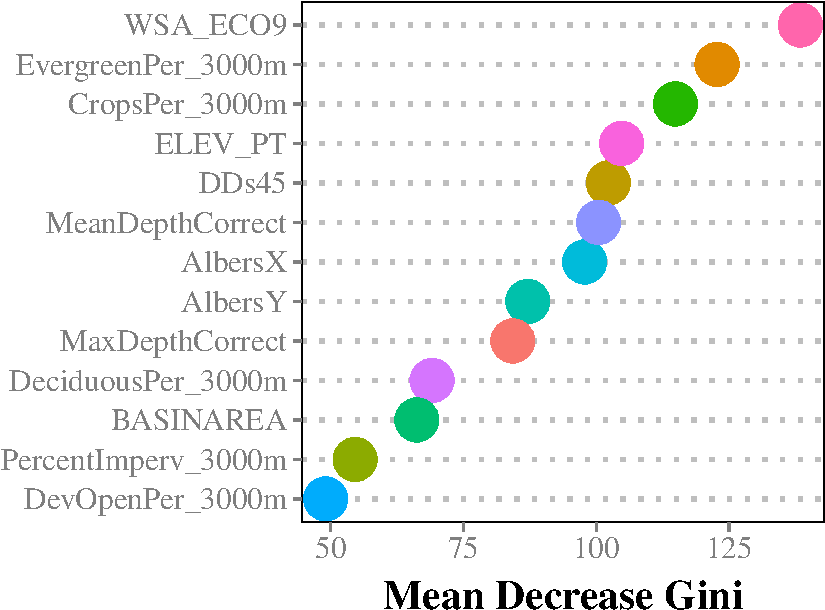
\includegraphics{./manuscript_files/figure-latex/Importance_Model6.pdf}
\caption{Importance plot for Model 6}
\end{figure}

\subsection{Associating Trophic State and
Cyanobacteria}\label{associating-trophic-state-and-cyanobacteria}

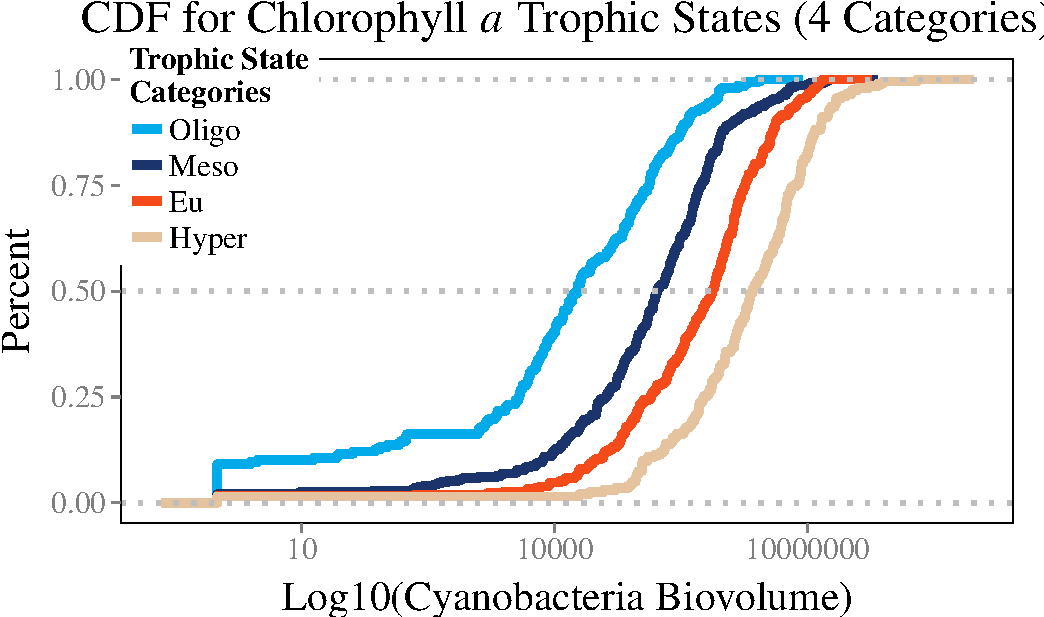
\includegraphics{./manuscript_files/figure-latex/ts_4_biov.pdf} \newpage
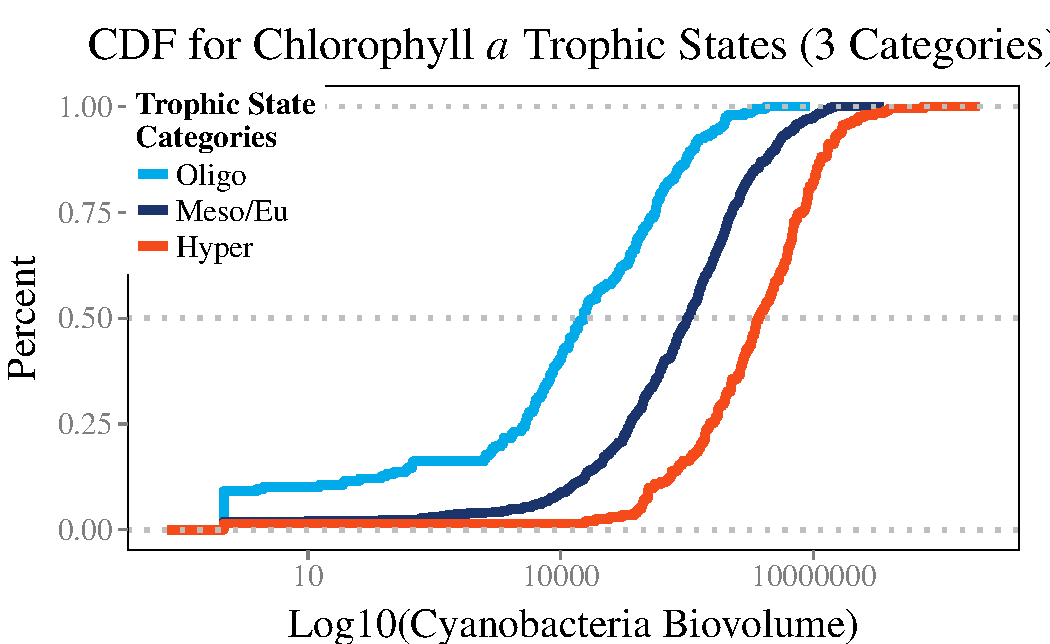
\includegraphics{./manuscript_files/figure-latex/ts_3_biov_cdf.pdf}
\newpage
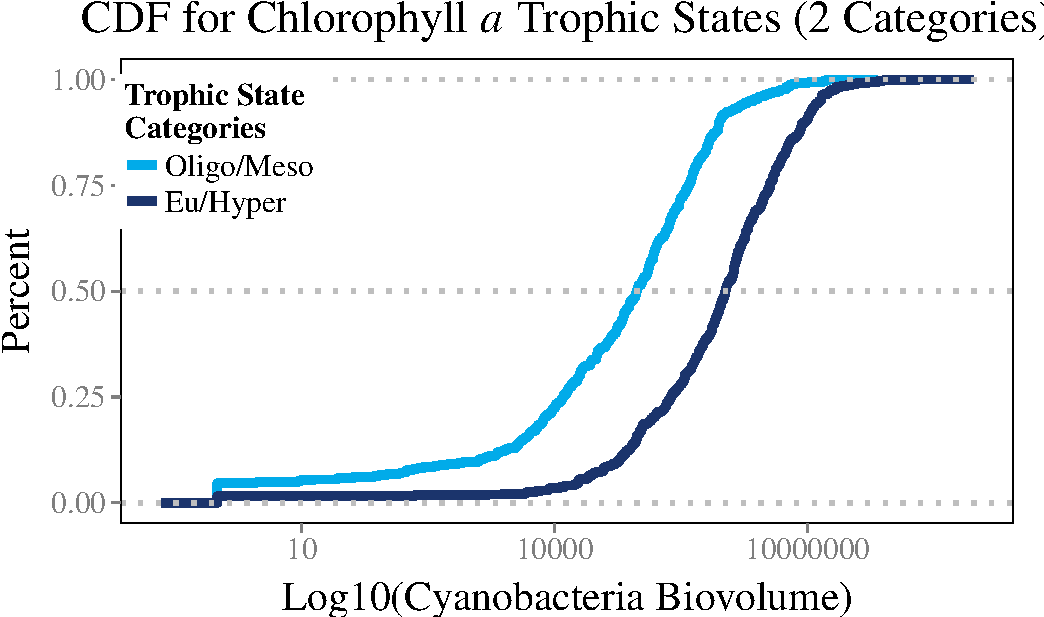
\includegraphics{./manuscript_files/figure-latex/ts_2_biov_cdf.pdf}
\newpage
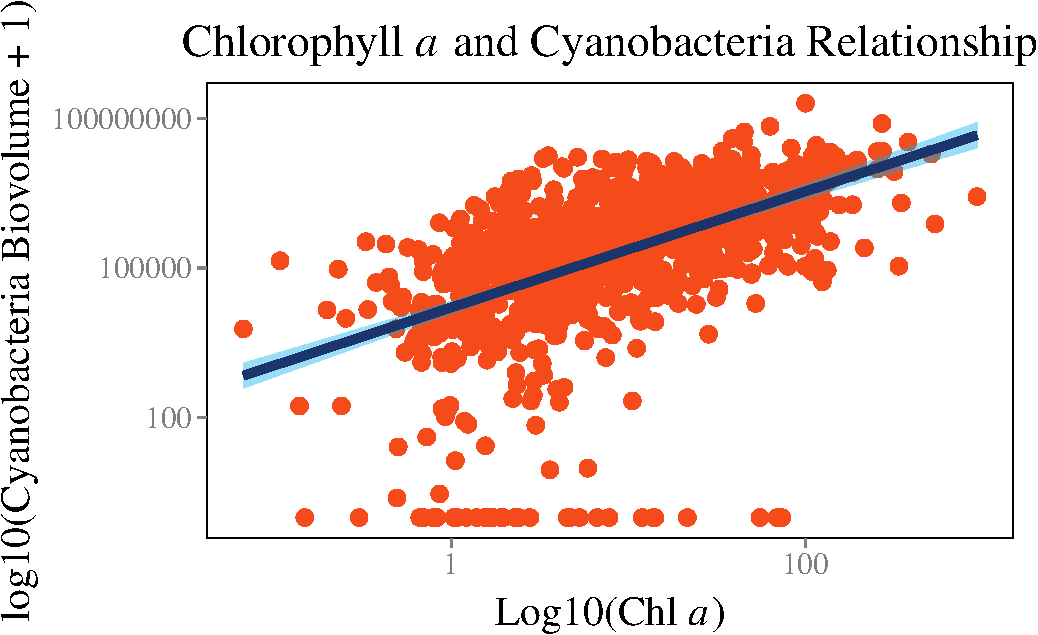
\includegraphics{./manuscript_files/figure-latex/scatterplot.pdf}

\newpage

\section*{References}\label{references}
\addcontentsline{toc}{section}{References}

Beaulieu, M., F. Pick, and I. Gregory-Eaves. 2013. Nutrients and water
temperature are significant predictors of cyanobacterial biomass in a
1147 lakes data set. Limnol. Oceanogr 58:1736--1746.

Breiman, L. 2001. Random forests. Machine learning 45:5--32.

Carlson, R. E. 1977. A trophic state index for lakes. Limnology and
oceanography 22:361--369.

Diaz-Uriarte, R. 2010. varSelRF: Variable selection using random
forests.

D{í}az-Uriarte, R., and S. A. De Andres. 2006. Gene selection and
classification of microarray data using random forest. BMC
bioinformatics 7:3.

Hollister, J. W. 2014. lakemorpho: Lake morphometry in r.

Hollister, J. W., and W. B. Milstead. In Preparation. National lake
morphometry dataset v1.0.

Hollister, J. W., W. B. Milstead, and M. A. Urrutia. 2011. Predicting
maximum lake depth from surrounding topography. PLoS ONE 6:e25764.

Hollister, J., and W. B. Milstead. 2010. Using gIS to estimate lake
volume from limited data. Lake and Reservoir Management 26:194--199.

Homer, C., C. Huang, L. Yang, B. Wylie, and M. Coan. 2004. Development
of a 2001 national land-cover database for the united states.
Photogrammetric Engineering \& Remote Sensing 70:829--840.

Liaw, A., and M. Wiener. 2002. Classification and regression by
randomForest. R News 2:18--22.

Smith, V. H. 1998. Cultural eutrophication of inland, estuarine, and
coastal waters. Pages 7--49 \emph{in} Successes, limitations, and
frontiers in ecosystem science. Springer.

Smith, V. H., S. B. Joye, R. W. Howarth, and others. 2006.
Eutrophication of freshwater and marine ecosystems. Limnology and
Oceanography 51:351--355.

Smith, V. H., G. D. Tilman, and J. C. Nekola. 1999. Eutrophication:
impacts of excess nutrient inputs on freshwater, marine, and terrestrial
ecosystems. Environmental pollution 100:179--196.

USEPA. 2009. National lakes assessment: a collaborative survey of the
nation's lakes. ePA 841-r-09-001. Office of Water; Office of Research;
Development, US Environmental Protection Agency Washington, DC.

Xian, G., C. Homer, and J. Fry. 2009. Updating the 2001 national land
cover database land cover classification to 2006 by using landsat
imagery change detection methods. Remote Sensing of Environment
113:1133--1147.

\end{document}
